\section{Resultat}

\begin{figure}
	\centering
	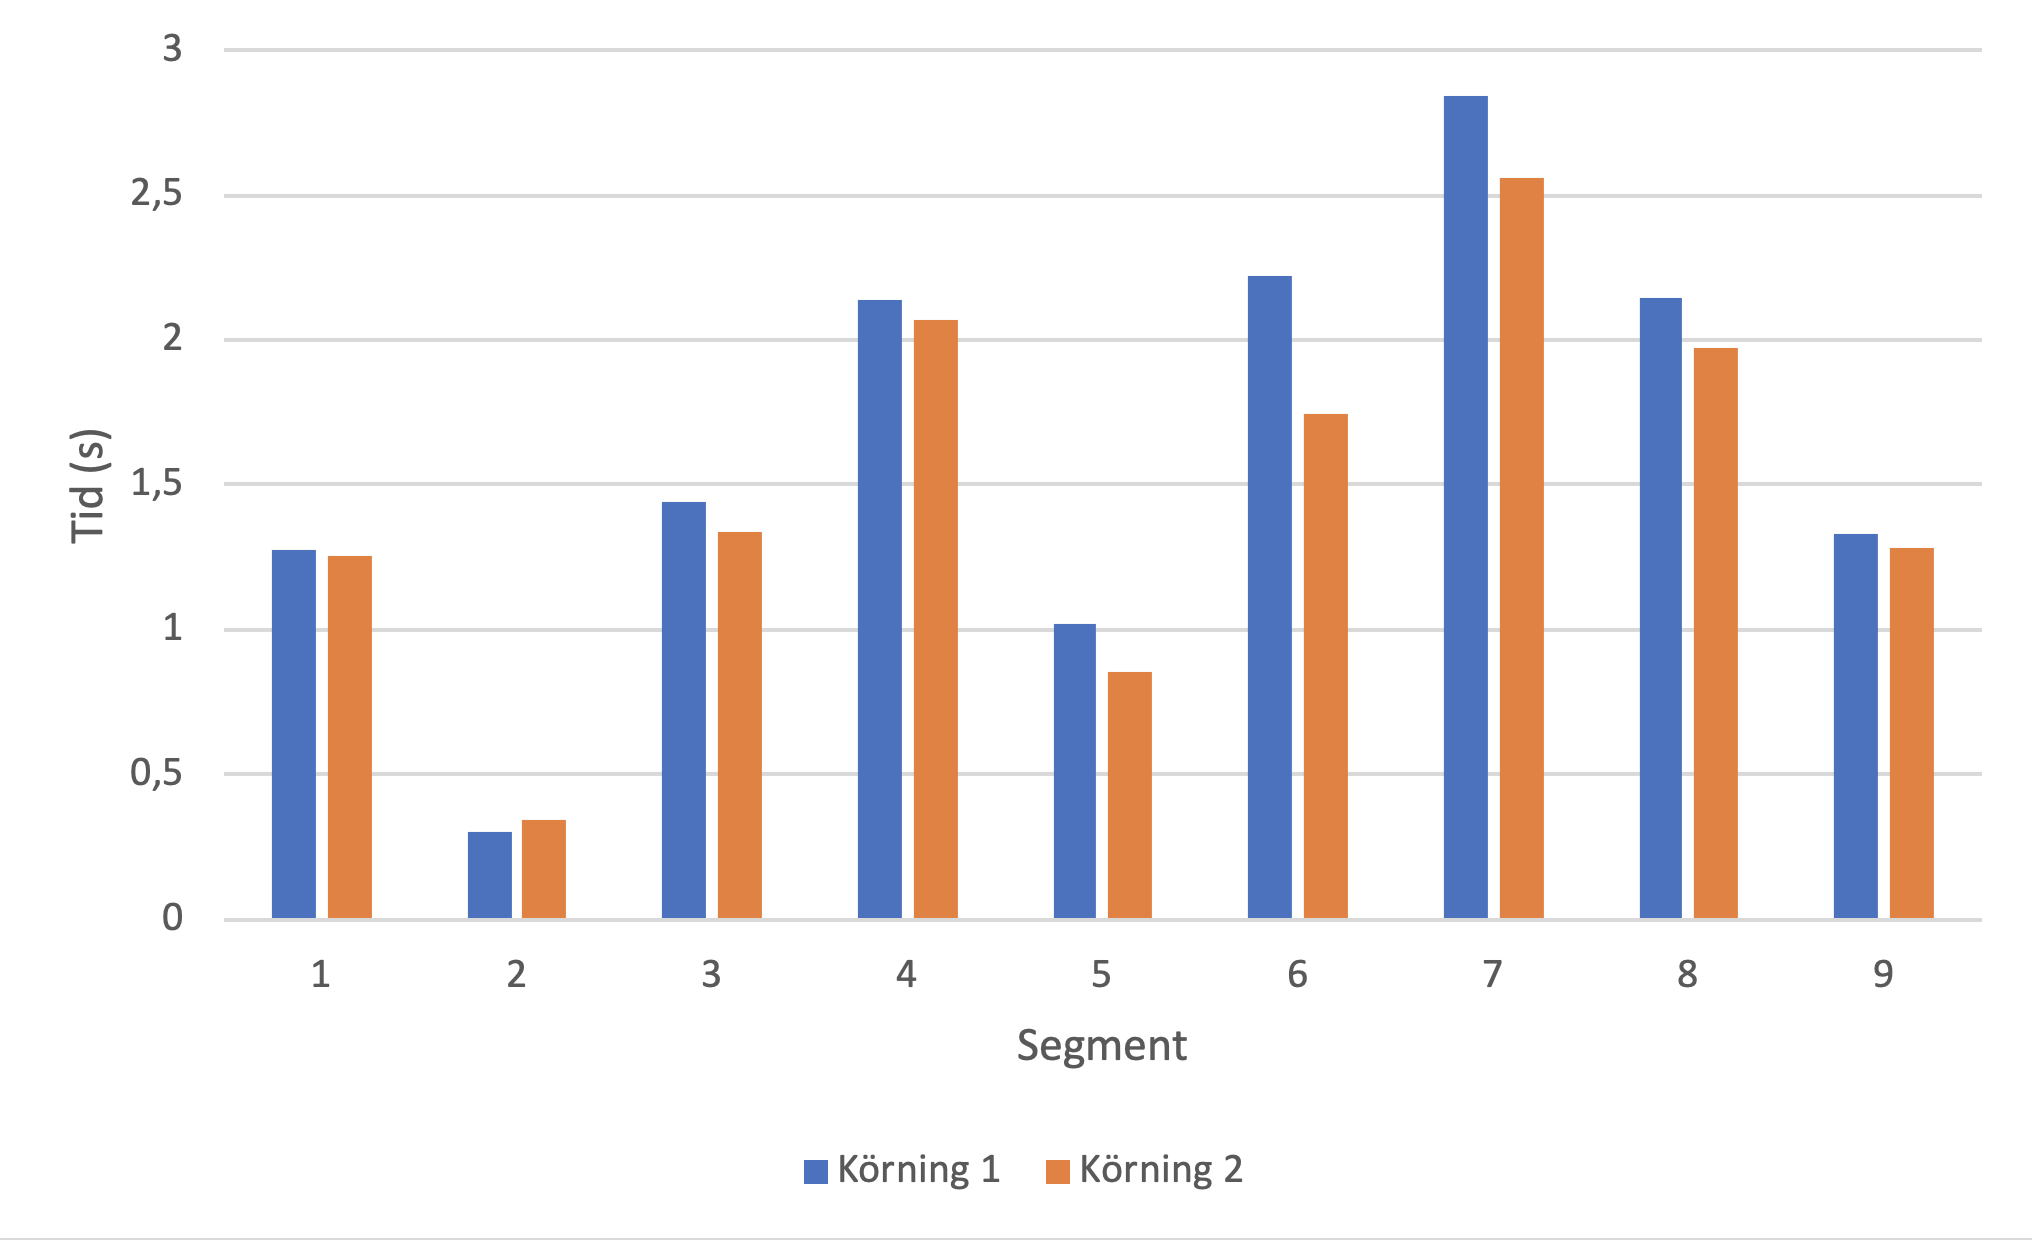
\includegraphics[width=0.5\linewidth]{Figures/segment_times}
	\caption{Genomsnittlig segmentstid för de två körningarna från redovisningen.}
	\label{fig:seg_times}
\end{figure}

\begin{figure}
	\centering
	\begin{tikzpicture}
		\begin{axis} [xmin=0, xmax=15.5,ymin=10,ymax=20, xlabel=Varv, ylabel={Tid (s)}, 
						legend pos=outer north east]
			\addplot+ [blue, mark options={blue}, mark=square*] table [col sep=comma, x index=0, y index = 1] {stats/lap.csv};
			\addlegendentry{Körning 1}
			\addplot+ [red, mark options={red}, mark=*] table [col sep=comma, x index=0, y index = 2] {stats/lap.csv};
			\addlegendentry{Körning 2}
		\end{axis}
	\end{tikzpicture}
  \caption{Varvtider för de två körningarna från redovisningen, inklusive
	kalibreringsvarven.}

	\vspace*{\floatsep}% https://tex.stackexchange.com/q/26521/5764

	\begin{tikzpicture}
		\begin{axis} [xmin=5.5, xmax=15.5,ymin=12,ymax=16, xlabel=Varv, ylabel={Tid (s)}, 
						legend pos=outer north east]
			\addplot+ [blue, mark options={blue}, mark=square*] table [col sep=comma, x index=0, y index = 1] {stats/lap.csv};
			\addlegendentry{Körning 1}
			\addplot[blue, domain=0:20] {13};
			\addlegendentry{Referenstid körning 1}
			\addplot+ [red, mark options={red}, mark=*] table [col sep=comma, x index=0, y index = 2] {stats/lap.csv};
			\addlegendentry{Körning 2}
			\addplot [red, domain=0:20] {14};
			\addlegendentry{Referenstid körning 2}
			\draw[dotted] (axis cs:0,12.5) -- (axis cs:16,12.5);
			\draw[dotted] (axis cs:0,13.5) -- (axis cs:16,13.5);
			\draw[dotted] (axis cs:0,14.5) -- (axis cs:16,14.5);
		\end{axis}
	\end{tikzpicture}
	\caption{Varvtider för de två körningarna från redovisningen, exklusive
	kalibreringsvarven.}
\end{figure}
